% Root file used ashow macros
\documentclass{beamer}
\usepackage{tikz}
\usetikzlibrary{calc}
\usepackage{xcolor}
\usepackage{multicol}
\usepackage{amsmath}

% ================================================================
% Answer-overlay helpers
% ================================================================
\newcommand{\ablank}[1]{%
  \alt<2>{\textcolor{red}{#1}}{\underline{\phantom{#1}}}%
}
\newcommand{\ashow}[1]{\uncover<2->{\textcolor{red}{\small #1}}}
\newcommand{\ashowq}[1]{\alt<2->{\textcolor{red}{\small #1}}{?}}

% Answers drawn straight on to a TikZ diagram, revealed on overlay 2 like \ashow.
% Space is reserved on overlay 1, so the diagram does not move between slides.
\usetikzlibrary{overlay-beamer-styles}
\tikzset{
  ans/.style     = {red, thick, visible on=<2->},
  ansfill/.style = {red!15, visible on=<2->},
  anslab/.style  = {red, font=\tiny, visible on=<2->},
}

\title{Fractions: Of Amounts \& Multiplying}
\author{}
\date{}

\begin{document}

\frame{\titlepage}

\begin{frame}{Contents}
\small
\begin{columns}[T]

\column{0.5\textwidth}
\textbf{Questions and short answers}
\begin{itemize}
  \item \hyperlink{q-st1}{\beamergotobutton{Starter 1}}
  \item \hyperlink{q-st2}{\beamergotobutton{Starter 2}}
  \item \hyperlink{q-st3}{\beamergotobutton{Starter 3}}
  \item \hyperlink{q-st4}{\beamergotobutton{Starter 4}}
  \item \hyperlink{q-st5}{\beamergotobutton{Starter 5}}
\end{itemize}

\column{0.5\textwidth}
\textbf{Worked solutions}
\begin{itemize}
  \item \hyperlink{work-st1}{\beamergotobutton{Starter 1}}
  \item \hyperlink{work-st2}{\beamergotobutton{Starter 2}}
  \item \hyperlink{work-st3}{\beamergotobutton{Starter 3}}
  \item \hyperlink{work-st4}{\beamergotobutton{Starter 4}}
  \item \hyperlink{work-st5}{\beamergotobutton{Starter 5}}
\end{itemize}

\end{columns}
\end{frame}

%------------------------------------------------
% STARTER 1
%------------------------------------------------
\begin{frame}{Starter 1}
\hypertarget{q-st1}{}

\vspace{-2em}

\begin{columns}

\column{0.25\textwidth}
\begin{center}
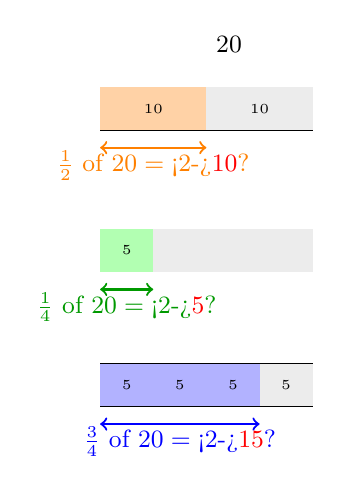
\begin{tikzpicture}[scale=0.9]

% Label for whole (20) above the top bar
\node[anchor=west] at (1.5,5.0) {\small $20$};

% Bar model for 1/2 of 20 (top)
\draw (0,3.8) rectangle (3,4.4);
\draw (1.5,3.8) -- (1.5,4.4);
\fill[orange!35] (0,3.8) rectangle (1.5,4.4);
\fill[gray!15] (1.5,3.8) rectangle (3,4.4);
\node at (0.75,4.1) {\tiny $10$};
\node at (2.25,4.1) {\tiny $10$};

\draw[<->, orange, thick] (0,3.55) -- (1.5,3.55);
\node[orange] at (0.75,3.3) {\small $\frac{1}{2}$ of $20 = \text{\ashowq{10}}$};

% Bar model for 1/4 of 20 (middle)
\draw (0,1.8) rectangle (3,2.4);
\foreach \x in {0.75,1.5,2.25} \draw (\x,1.8) -- (\x,2.4);
\fill[green!30] (0,1.8) rectangle (0.75,2.4);
\fill[gray!15] (0.75,1.8) rectangle (3,2.4);
\node at (0.375,2.1) {\tiny $5$};

\draw[<->, green!60!black, thick] (0,1.55) -- (0.75,1.55);
\node[green!60!black] at (0.375,1.3) {\small $\frac{1}{4}$ of $20 = \text{\ashowq{5}}$};

% Bar model for 3/4 of 20 (bottom)
\draw (0,-0.1) rectangle (3,0.5);
\foreach \x in {0.75,1.5,2.25} \draw (\x,-0.1) -- (\x,0.5);
\fill[blue!30] (0,-0.1) rectangle (2.25,0.5);
\fill[gray!15] (2.25,-0.1) rectangle (3,0.5);
\node at (0.375,0.2) {\tiny $5$};
\node at (1.125,0.2) {\tiny $5$};
\node at (1.875,0.2) {\tiny $5$};
\node at (2.625,0.2) {\tiny $5$};

\draw[<->, blue, thick] (0,-0.35) -- (2.25,-0.35);
\node[blue] at (1.125,-0.6) {\small $\frac{3}{4}$ of $20 = \text{\ashowq{15}}$};

\end{tikzpicture}
\end{center}

\column{0.75\textwidth}
\small
\begin{enumerate}
\begin{multicols}{2}
  \item Fully simplify: $\dfrac{18}{24}$ \ashow{$\dfrac{3}{4}$}
  \item Calculate: $2\dfrac{1}{3} + 1\dfrac{1}{2}$ \ashow{$=3\dfrac{5}{6}$}
\end{multicols}
  \item Using the bar models to the left:
  \[
    \tfrac{1}{2} \text{ of } 20 = \ablank{10} \qquad \tfrac{1}{4} \text{ of } 20 = \ablank{5} \qquad \tfrac{3}{4} \text{ of } 20 = \ablank{15}
  \]
  \item Calculate:
  \[
    \tfrac{1}{3} \text{ of } 24 \qquad \tfrac{2}{3} \text{ of } 24
  \]
  \ashow{$8$ and $16$}
  \item Fill in the blank: $\quad \dfrac{3}{4}$ of $\ablank{24} = 18$
  \item True or false? ``$\dfrac{1}{2}$ of $30 = 30 \div 2$.'' Explain your reasoning.
  \ashow{True. $\tfrac12$ of $30 = 15$ and $30 \div 2 = 15$.}
\begin{multicols}{2}
  \item Find $\dfrac{2}{5}$ of $35$. \ashow{$14$}
  \vspace{2em}
  \item A $60\,\text{cm}$ ribbon is cut. Amy takes $\dfrac{3}{4}$ of it. How long is her piece? \ashow{$45$ cm}
\end{multicols}
\end{enumerate}
\end{columns}
\end{frame}

\begin{frame}{Worked Solution: Starter 1, Question 1}
\hypertarget{work-st1}{}
\textbf{Question:} Fully simplify: \(\dfrac{18}{24}\).

\textbf{Worked Solution:}
Both \(18\) and \(24\) have highest common factor \(6\).
\[
\frac{18}{24}=\frac{18\div 6}{24\div 6}=\ablank{\frac{3}{4}}.
\]
\end{frame}

\begin{frame}{Worked Solution: Starter 1, Question 2}
\textbf{Question:} Calculate \(2\dfrac{1}{3}+1\dfrac{1}{2}\).

\textbf{Worked Solution:}
Write each mixed number as an improper fraction.
\[
2\frac{1}{3}+1\frac{1}{2}
=\frac{7}{3}+\frac{3}{2}
=\frac{14}{6}+\frac{9}{6}
=\frac{23}{6}
=\ablank{3\frac{5}{6}}.
\]
\end{frame}

\begin{frame}{Worked Solution: Starter 1, Question 3}
\textbf{Question:} Using the bar models, find \(\tfrac12\) of \(20\), \(\tfrac14\) of \(20\), and \(\tfrac34\) of \(20\).

\textbf{Worked Solution:}
The bar models show the whole split into equal parts. Reading the shaded portions:
\[
\frac12 \text{ of } 20=\ablank{10},\qquad
\frac14 \text{ of } 20=\ablank{5},\qquad
\frac34 \text{ of } 20=\ablank{15}.
\]
\end{frame}

\begin{frame}{Worked Solution: Starter 1, Question 4}
\textbf{Question:} Calculate \(\tfrac13\) of \(24\) and \(\tfrac23\) of \(24\).

\textbf{Worked Solution:}
\[
\frac13 \text{ of } 24 = 24\div3=\ablank{8}.
\]
Since \(\frac23\) is two of these parts,
\[
\frac23 \text{ of } 24 = 2\times8=\ablank{16}.
\]
\end{frame}

\begin{frame}{Worked Solution: Starter 1, Question 5}
\textbf{Question:} Fill in the blank: \(\frac34\) of a number is \(18\). Find the number.

\textbf{Worked Solution:}
Let the missing number be \(n\). One quarter is \(18\div3=6\), so the whole is \(4\times6=24\). Therefore
\[
\frac34 \text{ of } \ablank{24}=18.
\]
\end{frame}

\begin{frame}{Worked Solution: Starter 1, Question 6}
\textbf{Question:} True or false? ``\(\frac12\) of \(30=30\div2\).'' Explain your reasoning.

\textbf{Worked Solution:}
\[
\frac12\text{ of }30=\frac12\times30=\ablank{15},
\]
and
\[
30\div2=\ablank{15}.
\]
Both calculations give the same value, so the statement is \ablank{True}.
\end{frame}

\begin{frame}{Worked Solution: Starter 1, Question 7}
\textbf{Question:} Find \(\frac25\) of \(35\).

\textbf{Worked Solution:}
\[
\frac15\text{ of }35=7,\qquad
\frac25\text{ of }35=2\times7=\ablank{14}.
\]
\end{frame}

\begin{frame}{Worked Solution: Starter 1, Question 8}
\textbf{Question:} A \(60\,\text{cm}\) ribbon is cut. Amy takes \(\frac34\) of it. How long is her piece?

\textbf{Worked Solution:}
\[
\frac14\text{ of }60=15,\qquad
\frac34\text{ of }60=3\times15=45.
\]
Her piece is \ablank{$45$ cm}.
\end{frame}

%------------------------------------------------
% STARTER 2
%------------------------------------------------
\begin{frame}{Starter 2}
\hypertarget{q-st2}{}

\vspace{-2em}

\begin{columns}

\column{0.22\textwidth}
\begin{center}
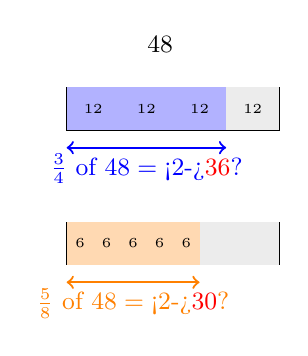
\begin{tikzpicture}[scale=0.9]

% Bar model for 3/4 of 48
\node[anchor=west] at (1, 5.5) {\small $48$};

\draw (0,4.3) rectangle (3,4.9);
\foreach \x in {0.75,1.5,2.25} \draw (\x,4.3) -- (\x,4.9);
\fill[blue!30] (0,4.3) rectangle (0.75,4.9);
\fill[blue!30] (0.75,4.3) rectangle (1.5,4.9);
\fill[blue!30] (1.5,4.3) rectangle (2.25,4.9);
\fill[gray!15] (2.25,4.3) rectangle (3,4.9);
\node at (0.375,4.6) {\tiny $12$};
\node at (1.125,4.6) {\tiny $12$};
\node at (1.875,4.6) {\tiny $12$};
\node at (2.625,4.6) {\tiny $12$};

\draw[<->, blue, thick] (0,4.05) -- (2.25,4.05);
\node[blue] at (1.125,3.75) {\small $\frac{3}{4}$ of $48 = \text{\ashowq{36}}$};


\draw (0,2.4) rectangle (3,3.0);
\foreach \x in {0.375,0.75,1.125,1.5,1.875,2.25,2.625} \draw (\x,2.4) -- (\x,3.0);
\fill[orange!30] (0,2.4) rectangle (1.875,3.0);
\fill[gray!15] (1.875,2.4) rectangle (3,3.0);
\node at (0.1875,2.7) {\tiny $6$};
\node at (0.5625,2.7) {\tiny $6$};
\node at (0.9375,2.7) {\tiny $6$};
\node at (1.3125,2.7) {\tiny $6$};
\node at (1.6875,2.7) {\tiny $6$};

\draw[<->, orange, thick] (0,2.15) -- (1.875,2.15);
\node[orange] at (0.9375,1.85) {\small $\frac{5}{8}$ of $48 = \text{\ashowq{30}}$};


\end{tikzpicture}
\end{center}

\column{0.78\textwidth}
\small
\begin{enumerate}
  \item Order smallest to largest: $\dfrac{3}{8},\ \dfrac{1}{2},\ \dfrac{5}{12}$ \ashow{$\dfrac{3}{8} < \dfrac{5}{12} < \dfrac{1}{2}$}
  \item Convert $\dfrac{17}{5}$ to a mixed number. \ashow{$3\dfrac{2}{5}$}
  \item Use the bar model to find $\dfrac{3}{4}$ of $48$ and $\dfrac{5}{8}$ of $48$. \ashow{$36$ and $30$}
  \item Calculate: $\quad \dfrac{5}{8}$ of $72$ \ashow{$=45$}
  \item $\dfrac{2}{3}$ of a class of $30$ are girls. How many boys are there? \ashow{$10$ boys}
  \item Rania says ``$\dfrac{3}{5}$ of $40 = 24$''. Is she correct? Show your working. \ashow{Yes; $\dfrac{3}{5}\times 40 = 24$.}

\begin{multicols}{2}
  \item Which is greater: \newline $\dfrac{3}{4}$ of $60$ or $\dfrac{4}{5}$ of $55$? \ashow{$\dfrac{3}{4}$ of $60$ ($=45$)}
  \item Fill in the blank:
  \[
    \frac{\ablank{5}}{8} \text{ of } 64 = 40
  \]
\end{multicols}
\end{enumerate}
\end{columns}
\end{frame}

\begin{frame}{Worked Solution: Starter 2, Question 1}
\hypertarget{work-st2}{}
\textbf{Question:} Order smallest to largest: \(\frac38,\ \frac12,\ \frac{5}{12}\).

\textbf{Worked Solution:}
Use common denominator \(24\).
\[
\frac38=\frac{9}{24},\quad
\frac{5}{12}=\frac{10}{24},\quad
\frac12=\frac{12}{24}.
\]
So the order is
\[
\ablank{\frac{3}{8}<\frac{5}{12}<\frac12}.
\]
\end{frame}

\begin{frame}{Worked Solution: Starter 2, Question 2}
\textbf{Question:} Convert \(\frac{17}{5}\) to a mixed number.

\textbf{Worked Solution:}
\(17\div5=3\) remainder \(2\), so
\[
\frac{17}{5}=3+\frac25=\ablank{3\frac25}.
\]
\end{frame}

\begin{frame}{Worked Solution: Starter 2, Question 3}
\textbf{Question:} Use the bar model to find \(\frac34\) of \(48\) and \(\frac58\) of \(48\).

\textbf{Worked Solution:}
For quarters: \(48\div4=12\), so \(\frac34\) of \(48=3\times12=\ablank{36}\).

For eighths: \(48\div8=6\), so \(\frac58\) of \(48=5\times6=\ablank{30}\).
\end{frame}

\begin{frame}{Worked Solution: Starter 2, Question 4}
\textbf{Question:} Calculate \(\frac58\) of \(72\).

\textbf{Worked Solution:}
\(72\div8=9\), so
\[
\frac58\times72=5\times9=\ablank{45}.
\]
\end{frame}

\begin{frame}{Worked Solution: Starter 2, Question 5}
\textbf{Question:} \(\frac23\) of a class of \(30\) are girls. How many boys are there?

\textbf{Worked Solution:}
If \(\frac23\) are girls, the fraction who are boys is
\[
1-\frac23=\frac13.
\]
So the number of boys is
\[
\frac13\times30=\ablank{10}.
\]
\end{frame}

\begin{frame}{Worked Solution: Starter 2, Question 6}
\textbf{Question:} Rania says ``\(\frac35\) of \(40=24\)''. Is she correct? Show your working.

\textbf{Worked Solution:}
\[
\frac15\text{ of }40=8,\qquad
\frac35\text{ of }40=3\times8=\ablank{24}.
\]
This matches the value in her statement, so Rania is \ablank{correct}.
\end{frame}

\begin{frame}{Worked Solution: Starter 2, Question 7}
\textbf{Question:} Which is greater: \(\frac34\) of \(60\) or \(\frac45\) of \(55\)?

\textbf{Worked Solution:}
\[
\frac34\times60=45,\qquad \frac45\times55=44.
\]
Since \(45>44\), the greater is \ablank{$\frac{3}{4}$ of $60$}.
\end{frame}

\begin{frame}{Worked Solution: Starter 2, Question 8}
\textbf{Question:} Fill in the blank: \(\frac{?}{8}\) of \(64=40\).

\textbf{Worked Solution:}
Let the missing numerator be \(n\). Then
\[
\frac{n}{8}\times64=8n.
\]
Since \(8n=40\), \(n=\ablank{5}\). Thus
\[
\frac{\ablank{5}}{8}\text{ of }64=40.
\]
\end{frame}

%------------------------------------------------
% STARTER 3
%------------------------------------------------
\begin{frame}{Starter 3}
\hypertarget{q-st3}{}

\vspace{-2em}

\begin{columns}

\column{0.25\textwidth}
\begin{center}
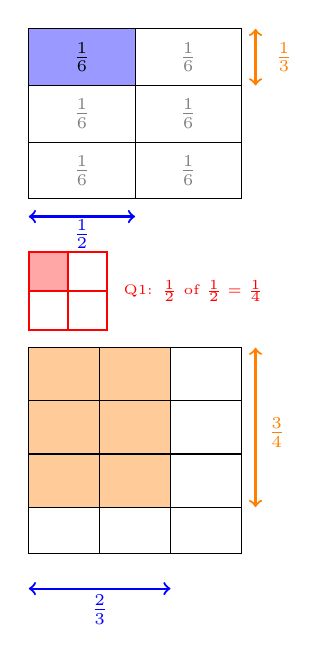
\begin{tikzpicture}[scale=0.9]

% Area model for 1/2 x 1/3
% Grid: 2 columns x 3 rows = 6 cells
\draw (0,2.5) rectangle (3,4.9);
% vertical line (halves)
\draw (1.5,2.5) -- (1.5,4.9);
% horizontal lines (thirds)
\draw (0,3.3) -- (3,3.3);
\draw (0,4.1) -- (3,4.1);

% shade 1 cell (top-left = 1/2 wide, 1/3 tall)
\fill[blue!40] (0,4.1) rectangle (1.5,4.9);

\node at (0.75,4.5) {\small $\frac{1}{6}$};
\node[gray] at (2.25,4.5) {\small $\frac{1}{6}$};
\node[gray] at (0.75,3.7) {\small $\frac{1}{6}$};
\node[gray] at (2.25,3.7) {\small $\frac{1}{6}$};
\node[gray] at (0.75,2.9) {\small $\frac{1}{6}$};
\node[gray] at (2.25,2.9) {\small $\frac{1}{6}$};

% labels on axes
\draw[<->, blue, thick] (0,2.25) -- (1.5,2.25);
\node[blue] at (0.75,2.0) {\small $\frac{1}{2}$};
\draw[<->, orange, thick] (3.2,4.1) -- (3.2,4.9);
\node[orange] at (3.6,4.5) {\small $\frac{1}{3}$};

% Area model for 2/3 x 3/4
\draw (0,-2.5) rectangle (3,0.4);
% shade 2/3 wide x 3/4 tall = 6 of 12 cells
\fill[orange!40] (0,-1.85) rectangle (2,0.4);

% vertical lines (thirds)
\draw (1,  -2.5) -- (1,  0.4);
\draw (2,  -2.5) -- (2,  0.4);
% horizontal lines (quarters)
\draw (0,-0.35) -- (3,-0.35);
\draw (0,-1.1) -- (3,-1.1);
\draw (0,-1.85) -- (3,-1.85);

% labels on axes
\draw[<->, blue, thick] (0,-3.0) -- (2,-3.0);
\node[blue] at (1,-3.3) {\small $\frac{2}{3}$};
\draw[<->, orange, thick] (3.2,0.4) -- (3.2,-1.85);
\node[orange] at (3.5,-0.8) {\small $\frac{3}{4}$};

% --- Q1 answer: 1/2 of 1/2 drawn as an area model ---
\fill[ansfill, red!35] (0,1.2) rectangle (0.55,1.75);
\draw[ans] (0,0.65) rectangle (1.1,1.75);
\draw[ans] (0.55,0.65) -- (0.55,1.75);
\draw[ans] (0,1.2) -- (1.1,1.2);
\node[anslab, right] at (1.2,1.2) {Q1: $\tfrac{1}{2}$ of $\tfrac{1}{2}=\tfrac{1}{4}$};
\end{tikzpicture}
\end{center}

\column{0.75\textwidth}
\small
\begin{enumerate}
  \item What is $\dfrac{1}{2}$ of $\dfrac{1}{2}$? Draw a picture to show your answer. \ashow{$\dfrac{1}{4}$}
  \item Use the area model on the left to calculate $\dfrac{1}{2} \times \dfrac{1}{3} = \dfrac{\ablank{1}}{\ablank{6}}$
  \item Use the second area model to calculate and simplify: $\dfrac{2}{3} \times \dfrac{3}{4} = \dfrac{\ablank{6}}{\ablank{12}} = \dfrac{\ablank{1}}{\ablank{2}}$
  \item Calculate:
  \[
    \frac{3}{5} \times \frac{5}{7}
  \]
  \ashow{$=\dfrac{3}{7}$}
  \item Simplify \textit{then} multiply: $\quad\dfrac{3}{9} \times \dfrac{4}{8}$ \ashow{$=\dfrac{1}{6}$}
  \item Find $\dfrac{3}{4}$ of $\dfrac{2}{5}$. What do you notice about ``of'' and ``$\times$''? \ashow{$\dfrac{3}{10}$; ``of'' means multiply.}
  \item Calculate: $1\dfrac{1}{2} \times \dfrac{1}{3}$\\[0.3em]
  (Hint: convert to improper first.) \ashow{$=\dfrac{1}{2}$}
\end{enumerate}
\end{columns}
\end{frame}

\begin{frame}{Worked Solution: Starter 3, Question 1}
\hypertarget{work-st3}{}
\textbf{Question:} What is \(\frac12\) of \(\frac12\)? Draw a picture to show your answer.

\textbf{Worked Solution:}
Multiply the numerators and the denominators:
\[
\frac12\times\frac12=\frac{1\times1}{2\times2}=\ablank{\frac14}.
\]

A picture:
\begin{center}
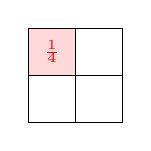
\begin{tikzpicture}[scale=0.6]
\fill[ansfill] (0,1) rectangle (1,2);
\draw (0,0) rectangle (2,2);
\draw (1,0)--(1,2);
\draw (0,1)--(2,1);
\node[anslab] at (0.5,1.5) {$\frac14$};
\end{tikzpicture}
\end{center}
\end{frame}

\begin{frame}{Worked Solution: Starter 3, Question 2}
\textbf{Question:} Use the area model on the left to calculate \(\frac12\times\frac13=\frac{\blank}{\blank}\).

\textbf{Worked Solution:}
From the area model, one of the six equal parts is shaded.
\[
\frac12\times\frac13=\frac{\ablank{1}}{\ablank{6}}.
\]
\end{frame}

\begin{frame}{Worked Solution: Starter 3, Question 3}
\textbf{Question:} Use the second area model to calculate and simplify:
\[
\frac23\times\frac34=\frac{\blank}{\blank}=\frac{\blank}{\blank}.
\]

\textbf{Worked Solution:}
\[
\frac23\times\frac34=\frac{\ablank{6}}{\ablank{12}}=\frac{\ablank{1}}{\ablank{2}}.
\]
\end{frame}

\begin{frame}{Worked Solution: Starter 3, Question 4}
\textbf{Question:} Calculate \(\frac35\times\frac57\).

\textbf{Worked Solution:}
Cancel the common factor \(5\).
\[
\frac35\times\frac57=\frac{3\times5}{5\times7}=\frac{15}{35}=\ablank{\frac37}.
\]
\end{frame}

\begin{frame}{Worked Solution: Starter 3, Question 5}
\textbf{Question:} Simplify \textit{then} multiply: \(\frac39\times\frac48\).

\textbf{Worked Solution:}
Simplify each fraction first.
\[
\frac39=\frac13,\qquad \frac48=\frac12
\]
so
\[
\frac39\times\frac48=\frac13\times\frac12=\ablank{\frac16}.
\]
\end{frame}

\begin{frame}{Worked Solution: Starter 3, Question 6}
\textbf{Question:} Find \(\frac34\) of \(\frac25\). What do you notice about ``of'' and ``\(\times\)''?

\textbf{Worked Solution:}
\[
\frac34\text{ of }\frac25=\frac34\times\frac25=\frac{3\times2}{4\times5}=\frac{6}{20}=\ablank{\frac{3}{10}}.
\]
This shows that \ablank{``of'' means the same as $\times$}.
\end{frame}

\begin{frame}{Worked Solution: Starter 3, Question 7}
\textbf{Question:} Calculate \(1\frac12\times\frac13\).

\textbf{Worked Solution:}
Convert to an improper fraction first:
\[
1\frac12=\frac32.
\]
Therefore
\[
1\frac12\times\frac13=\frac32\times\frac13=\frac{3}{6}=\ablank{\frac12}.
\]
\end{frame}

%------------------------------------------------
% STARTER 4
%------------------------------------------------
\begin{frame}{Starter 4}
\hypertarget{q-st4}{}

\vspace{-2em}

\begin{columns}

\column{0.22\textwidth}
\begin{center}
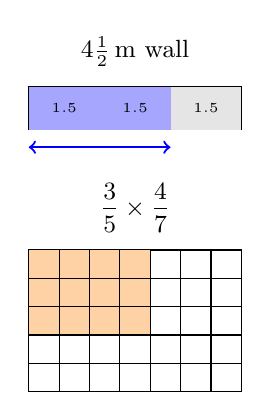
\begin{tikzpicture}[scale=0.9]

% Illustration: 2/3 of 4.5m wall
\node at (1.5, 5.3) {\small $4\tfrac{1}{2}$\,m wall};

\draw (0,4.2) rectangle (3,4.8);
\foreach \x in {1,2} \draw (\x,4.2) -- (\x,4.8);
\fill[gray!20] (0,4.2) rectangle (3,4.8);
\fill[blue!35] (0,4.2) rectangle (2,4.8);
\node at (0.5,4.5) {\tiny $1.5$};
\node at (1.5,4.5) {\tiny $1.5$};
\node at (2.5,4.5) {\tiny $1.5$};

\draw[<->, blue, thick] (0,3.95) -- (2,3.95);


% Area model reminder: 3/5 x 4/7
\node at (1.5,3.1) {\small $\dfrac{3}{5} \times \dfrac{4}{7}$};

\draw (0,0.5) rectangle (3,2.5);
\fill[orange!35] (0,1.3) rectangle (1.7143,2.5);

% 5 rows, 7 cols
\foreach \y in {0.9,1.3,1.7,2.1} \draw (0,\y) -- (3,\y);
\foreach \x in {0.4286,0.8571,1.2857,1.7143,2.1429,2.5714} \draw (\x,0.5) -- (\x,2.5);

\end{tikzpicture}
\end{center}

\column{0.78\textwidth}
\small
\begin{enumerate}
\begin{multicols}{3}
  \item Simplify: $\dfrac{24}{36}$ \ashow{$\dfrac{2}{3}$}
  \item $3\dfrac{1}{4} - 1\dfrac{2}{3}$ \ashow{$=1\dfrac{7}{12}$}
  \item $\dfrac{5}{6}$ of $42$ \ashow{$=35$}
\end{multicols}


  \item A wall is $4\dfrac{1}{2}$\,m long. A mural covers $\dfrac{2}{3}$ of it. Use the bar model to find the length of the mural. \ashow{$3$ m}


  \item Use the area model to calculate: $\dfrac{3}{5} \times \dfrac{4}{7} = \dfrac{\ablank{12}}{\ablank{35}}$

  \item Which is greater: $\dfrac{2}{3} \times \dfrac{3}{4}$, or $\dfrac{3}{4}$ of $\dfrac{2}{3}$? Explain. \ashow{They are equal ($\dfrac{1}{2}$).}

\begin{multicols}{2}
  \item Fill in the blank:
  \[
    \frac{3}{5} \times \ablank{\frac{2}{7}} = \frac{6}{35}
  \]
  \newline
  \item True or false? ``Multiplying two proper fractions always gives a smaller result than either fraction.'' Explain or give a counterexample. \ashow{True; e.g.\ $\dfrac{2}{3}\times\dfrac{3}{4}=\dfrac{1}{2}$, which is smaller than both.}
\end{multicols}
\end{enumerate}
\end{columns}
\end{frame}

\begin{frame}{Worked Solution: Starter 4, Question 1}
\hypertarget{work-st4}{}
\textbf{Question:} Simplify \(\frac{24}{36}\).

\textbf{Worked Solution:}
The highest common factor of \(24\) and \(36\) is \(12\).
\[
\frac{24}{36}=\frac{24\div12}{36\div12}=\ablank{\frac23}.
\]
\end{frame}

\begin{frame}{Worked Solution: Starter 4, Question 2}
\textbf{Question:} Calculate \(3\frac14-1\frac23\).

\textbf{Worked Solution:}
Convert to improper fractions:
\[
3\frac14=\frac{13}{4},\qquad 1\frac23=\frac53.
\]
Use a common denominator of \(12\):
\[
\frac{13}{4}-\frac53=\frac{39}{12}-\frac{20}{12}=\frac{19}{12}=\ablank{1\frac{7}{12}}.
\]
\end{frame}

\begin{frame}{Worked Solution: Starter 4, Question 3}
\textbf{Question:} Calculate \(\frac56\) of \(42\).

\textbf{Worked Solution:}
\(42\div6=7\), so
\[
\frac56\times42=5\times7=\ablank{35}.
\]
\end{frame}

\begin{frame}{Worked Solution: Starter 4, Question 4}
\textbf{Question:} A wall is \(4\frac12\) m long. A mural covers \(\frac23\) of it. Use the bar model to find the length of the mural.

\textbf{Worked Solution:}
\[
\frac23\times4\frac12=\frac23\times\frac92=\frac{18}{6}=\ablank{3\text{ m}}.
\]
\end{frame}

\begin{frame}{Worked Solution: Starter 4, Question 5}
\textbf{Question:} Use the area model to calculate \(\frac35\times\frac47=\frac{\blank}{\blank}\).

\textbf{Worked Solution:}
\[
\frac35\times\frac47=\frac{\ablank{12}}{\ablank{35}}.
\]
\end{frame}

\begin{frame}{Worked Solution: Starter 4, Question 6}
\textbf{Question:} Which is greater: \(\frac23\times\frac34\), or \(\frac34\) of \(\frac23\)? Explain.

\textbf{Worked Solution:}
\[
\frac23\times\frac34=\frac{6}{12}=\ablank{\frac12},
\]
and
\[
\frac34\text{ of }\frac23=\frac34\times\frac23=\frac{6}{12}=\ablank{\frac12}.
\]
Therefore \ablank{they are equal}.
\end{frame}

\begin{frame}{Worked Solution: Starter 4, Question 7}
\textbf{Question:} Fill in the blank:
\[
\frac35\times \blank = \frac{6}{35}.
\]

\textbf{Worked Solution:}
The missing fraction needs numerator \(6\div3=2\) and denominator \(35\div5=7\):
\[
\frac35\times\ablank{\frac{2}{7}}=\frac{6}{35}.
\]
\end{frame}

\begin{frame}{Worked Solution: Starter 4, Question 8}
\textbf{Question:} True or false? ``Multiplying two proper fractions always gives a smaller result than either fraction.'' Explain or give a counterexample.

\textbf{Worked Solution:}
\[
\frac23\times\frac34=\frac{6}{12}=\ablank{\frac12}.
\]
Since this product is smaller than both original fractions, the statement is \ablank{True}.
\end{frame}

%------------------------------------------------
% STARTER 5
%------------------------------------------------
\begin{frame}{Starter 5}
\hypertarget{q-st5}{}

\vspace{-2em}

\begin{columns}

\column{0.22\textwidth}
\begin{center}
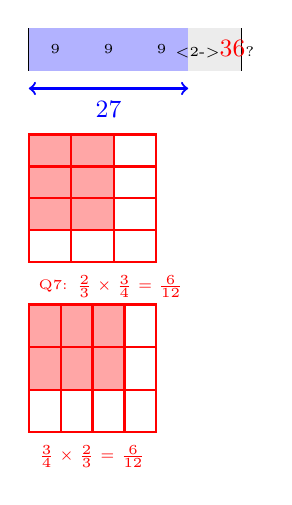
\begin{tikzpicture}[scale=0.9]

% Bar model: 3/4 of a number is 27

\draw (0,3.7) rectangle (3,4.3);
\foreach \x in {0.75,1.5,2.25} \draw (\x,3.7) -- (\x,4.3);
\fill[blue!30] (0,3.7) rectangle (2.25,4.3);
\fill[gray!15] (2.25,3.7) rectangle (3,4.3);
\node at (0.375,4.0) {\tiny $9$};
\node at (1.125,4.0) {\tiny $9$};
\node at (1.875,4.0) {\tiny $9$};
\node at (2.625,4.0) {\tiny \ashowq{36}};

\draw[<->, blue, thick] (0,3.45) -- (2.25,3.45);
\node[blue] at (1.125,3.15) {\small $27$};

% --- Q7 answer: the two area diagrams, each shading 6 of 12 cells ---
% 2/3 wide by 3/4 tall
\fill[ansfill, red!35] (0,1.45) rectangle (1.2,2.8);
\draw[ans] (0,1.0) rectangle (1.8,2.8);
\foreach \x in {0.6,1.2} \draw[ans] (\x,1.0) -- (\x,2.8);
\foreach \y in {1.45,1.9,2.35} \draw[ans] (0,\y) -- (1.8,\y);
\node[anslab, below right] at (0,0.95) {Q7: $\tfrac{2}{3}\times\tfrac{3}{4}=\tfrac{6}{12}$};
% 3/4 wide by 2/3 tall
\fill[ansfill, red!35] (0,-0.8) rectangle (1.35,0.4);
\draw[ans] (0,-1.4) rectangle (1.8,0.4);
\foreach \x in {0.45,0.9,1.35} \draw[ans] (\x,-1.4) -- (\x,0.4);
\foreach \y in {-0.8,-0.2} \draw[ans] (0,\y) -- (1.8,\y);
\node[anslab, below right] at (0,-1.45) {$\tfrac{3}{4}\times\tfrac{2}{3}=\tfrac{6}{12}$};
\end{tikzpicture}
\end{center}

\column{0.78\textwidth}
\small
\begin{enumerate}
\begin{multicols}{3}
  \item Simplify: $\dfrac{20}{30}$ \ashow{$\dfrac{2}{3}$}
  \item Simplify: $\dfrac{84}{108}$ \ashow{$\dfrac{7}{9}$}
\end{multicols}

  \item Convert $4\dfrac{3}{5}$ to an improper fraction. \ashow{$\dfrac{23}{5}$}


  \item Calculate: $2\dfrac{3}{4} + 1\dfrac{3}{5}$ \ashow{$=4\dfrac{7}{20}$}

  \item $\dfrac{3}{4}$ of a number is $27$. Use the bar model to find the whole number. \ashow{$36$}

  \item Jack spends $\dfrac{1}{3}$ of his pocket money on Monday and $\dfrac{1}{4}$ on Tuesday. What fraction remains? \ashow{$\dfrac{5}{12}$}

  \item A jug holds $1\dfrac{1}{2}$ litres. You fill $\dfrac{2}{3}$ of it. How many millilitres is that? \ashow{$1000$ mL}

  \item Show that $\dfrac{2}{3} \times \dfrac{3}{4} = \dfrac{3}{4} \times \dfrac{2}{3}$ using area diagrams.


\end{enumerate}
\end{columns}
\end{frame}

\begin{frame}{Worked Solution: Starter 5, Question 1}
\hypertarget{work-st5}{}
\textbf{Question:} Simplify \(\frac{20}{30}\).

\textbf{Worked Solution:}
The highest common factor of \(20\) and \(30\) is \(10\).
\[
\frac{20}{30}=\frac{20\div10}{30\div10}=\ablank{\frac23}.
\]
\end{frame}

\begin{frame}{Worked Solution: Starter 5, Question 2}
\textbf{Question:} Simplify \(\frac{84}{108}\).

\textbf{Worked Solution:}
The highest common factor of \(84\) and \(108\) is \(12\).
\[
\frac{84}{108}=\frac{84\div12}{108\div12}=\ablank{\frac79}.
\]
\end{frame}

\begin{frame}{Worked Solution: Starter 5, Question 3}
\textbf{Question:} Convert \(4\frac35\) to an improper fraction.

\textbf{Worked Solution:}
\[
4=\frac{20}{5},\qquad 4\frac35=\frac{20}{5}+\frac35=\ablank{\frac{23}{5}}.
\]
\end{frame}

\begin{frame}{Worked Solution: Starter 5, Question 4}
\textbf{Question:} Calculate \(2\frac34+1\frac35\).

\textbf{Worked Solution:}
\[
2\frac34=\frac{11}{4},\qquad 1\frac35=\frac85.
\]
Use a common denominator of \(20\):
\[
\frac{11}{4}+\frac85=\frac{55}{20}+\frac{32}{20}=\frac{87}{20}=\ablank{4\frac{7}{20}}.
\]
\end{frame}

\begin{frame}{Worked Solution: Starter 5, Question 5}
\textbf{Question:} \(\frac34\) of a number is \(27\). Use the bar model to find the whole number.

\textbf{Worked Solution:}
If three quarters is \(27\), one quarter is
\[
27\div3=\ablank{9}.
\]
So the whole number is
\[
4\times9=\ablank{36}.
\]
\end{frame}

\begin{frame}{Worked Solution: Starter 5, Question 6}
\textbf{Question:} Jack spends \(\frac13\) of his pocket money on Monday and \(\frac14\) on Tuesday. What fraction remains?

\textbf{Worked Solution:}
Total spent:
\[
\frac13+\frac14=\frac{4}{12}+\frac{3}{12}=\frac{7}{12}.
\]
Fraction remaining:
\[
1-\frac{7}{12}=\ablank{\frac{5}{12}}.
\]
\end{frame}

\begin{frame}{Worked Solution: Starter 5, Question 7}
\textbf{Question:} A jug holds \(1\frac12\) litres. You fill \(\frac23\) of it. How many millilitres is that?

\textbf{Worked Solution:}
\(1\frac12\) litres \(=1500\) mL.
\[
\frac23\times1500=\ablank{1000\text{ mL}}.
\]
\end{frame}

\begin{frame}{Worked Solution: Starter 5, Question 8}
\textbf{Question:} Show that \(\frac23\times\frac34=\frac34\times\frac23\) using area diagrams.

\textbf{Worked Solution:}
The two area diagrams below each shade \(6\) of \(12\) cells, showing the products are equal.

\begin{center}
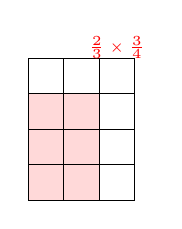
\begin{tikzpicture}[scale=0.45]
% 2/3 wide by 3/4 tall: 3 columns, 4 rows
\fill[ansfill] (0,0) rectangle (2,3);
\draw (0,0) rectangle (3,4);
\foreach \x in {1,2} \draw (\x,0) -- (\x,4);
\foreach \y in {1,2,3} \draw (0,\y) -- (3,\y);
\node[anslab] at (2.5,4.3) {$\frac23\times\frac34$};
\end{tikzpicture}
\hspace{1cm}
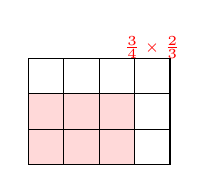
\begin{tikzpicture}[scale=0.45]
% 3/4 wide by 2/3 tall: 4 columns, 3 rows
\fill[ansfill] (0,0) rectangle (3,2);
\draw (0,0) rectangle (4,3);
\foreach \x in {1,2,3} \draw (\x,0) -- (\x,3);
\foreach \y in {1,2} \draw (0,\y) -- (4,\y);
\node[anslab] at (3.5,3.3) {$\frac34\times\frac23$};
\end{tikzpicture}
\end{center}

\[
\ablank{\frac23\times\frac34=\frac34\times\frac23}.
\]
\end{frame}

\end{document}